\chapter*{Introduction}
\addcontentsline{toc}{chapter}{1. Introduction} % Manual index entry
% Hablar de la empresa
% Hablar del objetivo del trabajo
% Comentar la estructura del documento

PRUEBA GLOSARIO: \gls{tempo}$^{(*)}$


En el mundo actual, donde la eficiencia y la toma de decisiones estratégicas marcan la diferencia entre avanzar o quedarse atrás, la gestión de tareas dentro de una empresa adquiere un papel fundamental.
Muchas veces, detrás de un buen producto o servicio, hay una planificación precisa, una coordinación cuidada y un aprovechamiento óptimo de los recursos disponibles.
En este contexto, las matemáticas, y más concretamente la optimización, se convierten en una herramienta poderosa para transformar la complejidad en soluciones claras y aplicables.

Este trabajo surge con la intención de tender un puente entre el conocimiento teórico y su aplicación práctica en el entorno empresarial.
Hemos elegido como caso de estudio la empresa Intercrop, ubicada en Cartagena, especializada en el sector agroalimentario.
Intercrop destaca por su compromiso con la sostenibilidad y la innovación en la producción agrícola, pero como toda empresa, se enfrenta a retos logísticos y organizativos que requieren soluciones inteligentes.
Intercrop no solo opera a nivel nacional, sino que también mantiene una estrecha relación con el mercado internacional. 
Exporta una parte importante de su producción a distintos países europeos, lo que exige altos estándares de calidad, cumplimiento riguroso de plazos y una logística bien estructurada.
Esta dimensión internacional añade complejidad a su gestión operativa, ya que debe coordinar las tareas agrícolas con los calendarios de transporte, las exigencias fitosanitarias y los compromisos comerciales en el extranjero.
Todo ello convierte a esta empresa en un entorno especialmente interesante para aplicar herramientas de optimización que ayuden a mejorar la planificación y la eficiencia en un contexto real y exigente.

A través de este proyecto, abordaremos el problema de planificación de tareas dentro de la empresa. La meta es diseñar un modelo de optimización que permita organizar de forma eficiente las actividades,
 considerando las restricciones del entorno real: tiempos, recursos limitados, dependencias entre tareas y otros factores logísticos.
Este proceso nos permitirá no solo aportar una propuesta de mejora a la empresa, sino también aplicar de forma práctica los conceptos matemáticos aprendidos en el aula, especialmente en lo que respecta a programación lineal y optimización.
\vspace{10mm}
\begin{figure}[ht!]
    \centering
    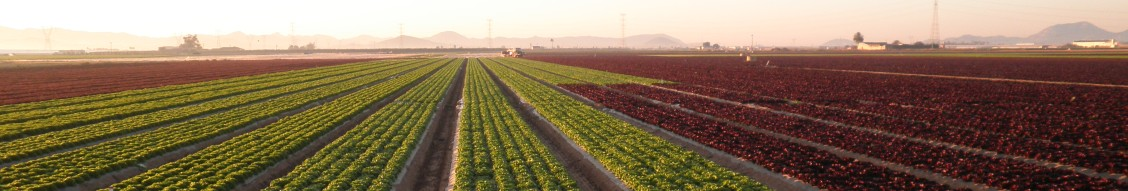
\includegraphics[width=1\textwidth]{img/campitos_lindos.jpeg}
    %\caption{Intercrop, empresa de referencia para el estudio de planificación de tareas agrícolas.}
    \label{fig:campitos_lindos}
\end{figure}

\chapter*{Problem Statement}
\addcontentsline{toc}{chapter}{2. Problem Statement} % Manual index entry
% Explicación en "leguaje natural" del problema
% Simplificaciones
% Descripción de las tareas

La planificación de tareas en el entorno agrícola representa un desafío logístico y operativo considerable,
especialmente en empresas que operan bajo un modelo de producción bajo pedido, como es el caso de Intercrop.
Esta empresa, situada en Cartagena y especializada en productos hortícolas, organiza su producción en función de la demanda estacional.
Durante la campaña de verano, se establecen con antelación tanto la cantidad de kilogramos de producto que se deben suministrar como las fechas específicas de entrega.
Esto implica que toda la planificación de cultivo, desarrollo, cosecha y distribución debe estar ajustada con precisión para cumplir los plazos,
garantizar la calidad del producto fresco (con una vida útil de entre siete y diez días) y minimizar los costes operativos.

El objetivo de este trabajo es abordar, desde un enfoque matemático y práctico, el problema de planificación de tareas agrícolas en el entorno real de esta empresa.
Para ello, nos centraremos en dos cultivos principales: lechuga y espinaca, cada uno con dos variantes específicas.
\begin{itemize}
    \item \textbf{Lechuga}: se cultiva en dos variedades, una de hoja rizada (Apollo, Fig. \ref{fig:apollo}) y otra de hoja lisa (Knox Cos, Fig. \ref{fig:knox}). La lechuga de hoja rizada es más delicada y requiere un cuidado especial. Por su parte, la lechuga de hoja lisa es más resistente y se adapta mejor a condiciones menos precisas.
    \item \textbf{Espinaca}: también se cultiva en dos variedades, una de hoja pequeña (Baby Spinach, Fig. \ref{fig:baby}) y otra de hoja mediana (Teen Spinach, Fig. \ref{fig:teen}). En cuanto a las difere en el tratamiento, no se encuentran ambios sustanciales en el cuidado.
\end{itemize}

\begin{figure}[ht!]
    \centering

    \begin{minipage}[b]{0.45\textwidth}
        \centering
        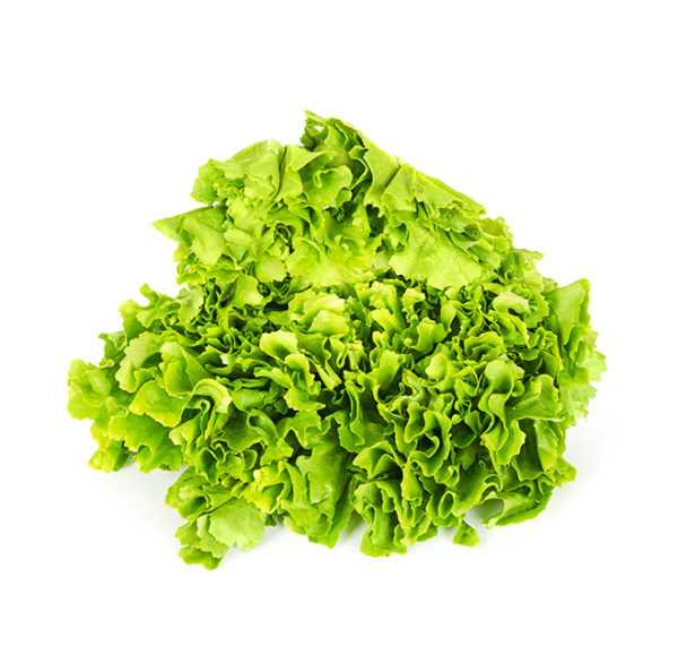
\includegraphics[width=0.7\textwidth]{img/lechuga_apollo.png}
        \caption{Variedad Lechuga Apollo.}
        \label{fig:apollo}
    \end{minipage}
    \hfill
    \begin{minipage}[b]{0.45\textwidth}
        \centering
        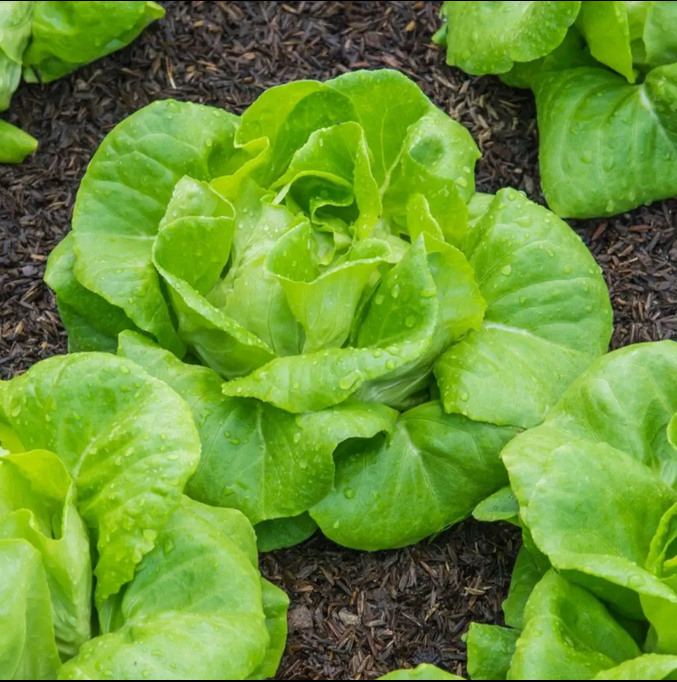
\includegraphics[width=0.6\textwidth]{img/lechuga_knox.png}
        \caption{Variedad Lechuga Knox Cos.}
        \label{fig:knox}
    \end{minipage}

\end{figure}

\begin{figure}[ht!]
    \centering

    \begin{minipage}[b]{0.45\textwidth}
        \centering
        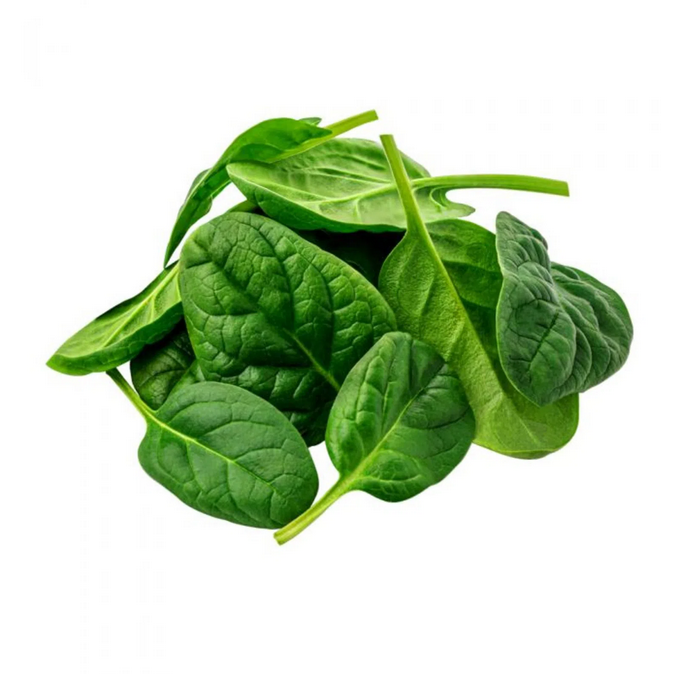
\includegraphics[width=0.7\textwidth]{img/baby_spinach.png}
        \caption{Variedad Baby Spinach.}
        \label{fig:baby}
    \end{minipage}
    \hfill
    \begin{minipage}[b]{0.45\textwidth}
        \centering
        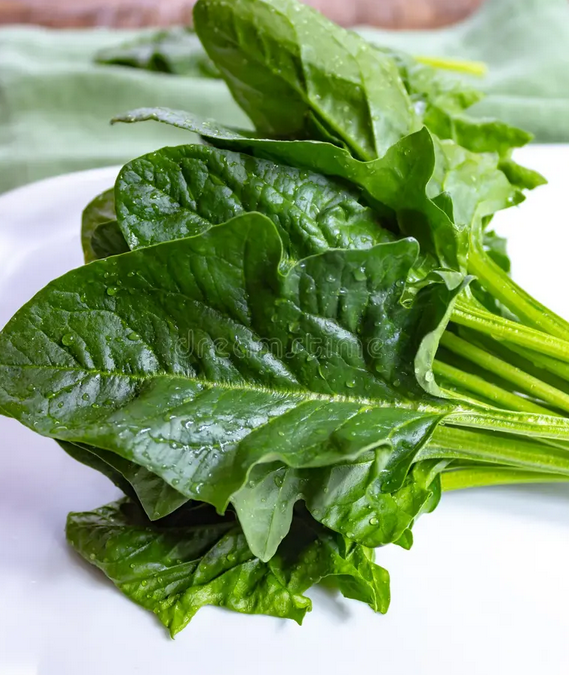
\includegraphics[width=0.6\textwidth]{img/teen_spinach.png}
        \caption{Variedad Teen Spinach.}
        \label{fig:teen}
    \end{minipage}

\end{figure}


Antes de pasar a desglosar las tareas que engloban el poceso de cultivo, es importante destacar una diferencia fundamental entre ambos productos.
La lechuga se trabaja mediante plantación: las semillas se envían a un semillero y posteriormente se trasplantan las plántulas al campo. 
En el caso de la espinaca, se utiliza el método de siembra directa, introduciendo las semillas directamente en la tierra.
Debido al difierente proceder de ambos métodos, cada cultivo tendrá sus tiempos y necesidades específicas, lo que influirá en la planificación de las tareas.




% REVISADO HASTA AQUI















\newpage
Con este objetivo, hemos centrado nuestro estudio en dos fincas concretas, cada una dedicada al cultivo de un producto diferente: lechuga y espinaca.
La elección de estos dos productos no ha sido aleatoria; se debe a las marcadas diferencias en sus necesidades de cuidado y manejo.
De hecho, es en estas diferencias donde se concentran gran parte de las particularidades de las líneas de trabajo dentro de la empresa.
Para enriquecer aún más el modelo y hacerlo más representativo, hemos considerado dos variantes dentro de cada uno de estos productos, lo que nos permite capturar con mayor fidelidad la diversidad de cultivos con la que trabaja Intercrop en la práctica.

En cada finca se lleva a cabo una secuencia de tareas específicas necesarias para completar el ciclo productivo de forma adecuada. Estas tareas, que constituyen el núcleo del proceso agrícola, son las siguientes:
\begin{enumerate}
    \item Preparación de la tierra: conjunto de labores inicales donde se rompe y voltea la tierra para airearla, y se abona para dejarla preparada adecuadamente antes del cultivo.
    \item Creación de mesetas: mediante maquinaria especializada, se organizan las superficies de cultivo en mesetas 
    \item Colocar papel: se instalan láminas que impiden el crecimiento de malas hierbas, lo que reduce la competencia con el cultivo principal.
    \item Sembrar o plantar: según el tipo de variante, se introducen semillas directamente o se plantan brotes previamente cultivados por una empresa externa.
    \item Riego: instalación de sistemas de riego por aspersión en las laderas de las mesetas, necesarios para el mantenimiento del cultivo.
    \item Colocación de arquillos: se instalan arcos metálicos sobre los cultivos para dar soporte a la protección posterior.
    \item Poner malla: se cubren los arquillos con una malla de poliamida que protege los cultivos y ayuda a mantener la temperatura adecuada para su desarrollo.
    \item Quitar malla: una vez que el cultivo ha madurado, se retira la malla protectora.
    \item Quitar arquillos: tras la retirada de la malla, se procede a desmontar los arquillos metálicos.
    \item Quitar riego: se desmonta el sistema de riego instalado previamente.
    \item Recogida de cosecha: proceso final de recolección, que puede realizarse manualmente (con operarios que colocan los productos en cajas) o de forma automatizada.
\end{enumerate}

Cada una de estas tareas requiere el uso de maquinaria diferente y, en consecuencia, se ejecutan a velocidades distintas.
La empresa nos proporcionó inicialmente los datos de velocidad en términos de kilómetros por hora (km/h), pero para simplificar el tratamiento y adaptarlo al enfoque del modelo,
hemos traducido dichas velocidades a unidades de mesetas por hora, lo cual permite un análisis más directo de la producción por unidad de superficie en cada finca.

Asimismo, hemos realizado una simplificación adicional asumiendo que ambas fincas tienen un tamaño medio y uniforme, lo que facilita la estandarización de los cálculos y permite aplicar el mismo esquema de planificación a cada caso.
También hemos considerado que existen dos grupos de trabajo totalmente independientes, uno para cada producto, cada uno con su propia maquinaria y sin interferencias directas entre ellos.
Esta separación nos permite modelar cada línea de trabajo por separado, aunque posteriormente estudiaremos la interacción indirecta a través del uso compartido de espacios y tiempos.

Otra suposición importante ha sido establecer que las condiciones de trabajo son ideales: no existen imprevistos derivados del clima ni averías en la maquinaria.
Esta "atmósfera idílica" nos permite centrarnos en el análisis estructural del problema de planificación sin tener que introducir incertidumbres que, aunque reales, complejizarían el modelo en exceso para una primera aproximación.

Durante nuestra visita a las instalaciones de Intercrop, observamos un aspecto crítico que nos llevó a la definición del objetivo del presente trabajo:
en numerosas ocasiones, los equipos de trabajo deben esperar a que otros terminen su tarea antes de poder comenzar la suya, especialmente cuando varias tareas se solapan en la misma meseta.
Este solapamiento produce horas muertas, es decir, periodos en los que un grupo de trabajo no puede avanzar, aunque el tiempo siga transcurriendo y se sigan generando costes laborales y operativos.
Estas horas improductivas son especialmente problemáticas porque aumentan el coste de producción sin aportar valor añadido, afectando directamente a la eficiencia de la empresa.

El objetivo central de este trabajo, por tanto, es minimizar el número de horas muertas entre los grupos de trabajo, mediante una planificación adecuada de las tareas.
A través del desarrollo de un modelo matemático de optimización, pretendemos encontrar una asignación y secuencia de tareas que reduzca los tiempos de espera y, por tanto,
mejore el aprovechamiento de los recursos humanos y técnicos disponibles. En definitiva, buscamos una solución que, aun partiendo de una simplificación del problema real, permita extraer conclusiones prácticas y proponer mejoras concretas en la gestión operativa de la empresa.



\chapter*{Formulation}
\addcontentsline{toc}{chapter}{3. Formulation} % Manual index entry

% Variables
% Funcion objetivo
% Restricciones

\chapter*{Data}
\addcontentsline{toc}{chapter}{4. Data} % Manual index entry
% Explicación de los datos
% Tablas

Durante nuestra visita a la empresa, recopilamos todos los datos necesarios para nuestro análisis. 
Posteriormente, la empresa nos facilitó la información que habíamos solicitado.

Para nuestro estudio, asumimos que las fincas tienen una forma rectangular, con dimensiones promedio
 de 100 x 300 metros. Cada meseta de cultivo mide 1.6 metros de ancho, con surcos laterales de 0.4 metros
  para permitir el paso de la maquinaria. Esto implica que cada camino tendrá unas dimensiones de 2 x 300 metros.
   En consecuencia, en cada finca disponemos de 50 caminos y sus respectivas 50 mesetas para el cultivo.

Dado que todas las tareas están mecanizadas, es fundamental considerar la velocidad de las máquinas utilizadas en el
 proceso. Aunque la empresa nos proporcionó estos datos en kilómetros por hora (km/h), para facilitar nuestra formulación 
 convertimos las unidades a caminos por hora.
 
 \begin{table}[ht!]
    \begin{tabular}{lclll}
    \textbf{TASK}      & \multicolumn{1}{l}{\textbf{SPEED}} \\
    Soil preparation   & 2                                  \\
    Install paper      & 4                                  \\
    Plant              & 3                                  \\
    Sow                & 4                                  \\
    Install irrigation & 3                                  \\
    Install hoops      & 3                                  \\
    Install mesh       & 3                                  \\
    Remove irrigation  & 3                                  \\
    Remove mesh        & 4                                  \\
    Remove hoops       & 3                                  \\
    Harvest seeds      & 3                                  \\
    Harvest plants     & 2                                            
    \end{tabular}
    \end{table}

Nuestra planificación está diseñada para organizar un mes de trabajo. Considerando una jornada laboral de 8 horas diarias, 
trabajamos con un total de 240 horas al mes.

Por otro lado, los trabajadores se incorporan a la campaña de manera escalonada. Cada uno de ellos está especializado en una 
tarea específica, lo que da lugar a la formación de grupos de trabajo especializados. El número de trabajadores por grupo varía 
en función de la tarea asignada.



\chapter*{Code}
\addcontentsline{toc}{chapter}{5. Code} % Manual index entry\addcontentsline{toc}{chapter}{5. Code} % Manual index entry
% Explicación del código
% Código

\chapter*{Results}
\addcontentsline{toc}{chapter}{6. Results} % Manual index entry
% Explicación de los resultados
% Tablas
% Gráficos

\chapter*{Conclusion}
\addcontentsline{toc}{chapter}{7. Conclusion} % Manual index entry


\newpage
------------------------------

- Topo
- Apero
- Siembra
- Plantación
- Meseta
- Arquillo
- Malla
- Papel
- Farm lanes: caminos entre las mesetas para el paso de la maquinaria.
- Semillero
